\documentclass[12pt, letterpaper]{article}

\usepackage{placeins}
\usepackage{appendix}
\usepackage{todonotes}
\usepackage{graphicx}
\usepackage{titling}
\usepackage{xcolor}

% Palatino font for text and math 
\usepackage{mathpazo}
% Bera Mono font for monospace text (code blocks)
\usepackage[scaled]{beramono}
\usepackage[T1]{fontenc}

% Syntax highlighting for Verilog code snippets
\usepackage{listings}
\definecolor{vgreen}{RGB}{104,180,104}
\definecolor{vblue}{RGB}{49,49,255}
\definecolor{vorange}{RGB}{255,143,102}

\lstdefinestyle{verilog-style}
{
    language=Verilog,
    basicstyle=\small\ttfamily,
    keywordstyle=\color{vblue},
    identifierstyle=\color{black},
    commentstyle=\color{vgreen},
    tabsize=2,  % small tab size so code doesn't run off the right-hand-side margin
    literate=*{:}{:}1
}







\title{Lab \# 4 - 5: \textbf{Adding Register File to ALU, Adding Data Memory to the Datapath}}

% I just copied your name as it appeared in gmail - Tim
\author{Group \# \textbf{14}:\\ Jin Hyeong Kim \and\\ Timothy VanSlyke}


\begin{document}

\begin{titlepage}
	\begin{center}
		{\Large
			\textbf{Northeastern University}\\
			~\\
			Department of Electrical and Computer Engineering\\ 
		}

		\vfill

		{\large
			EECE2323: \textbf{Digital Systems Design Lab}\\
			~\\
			Lecturer: \textbf{Dr. Emad Aboelela}\\
			~\\
			TAs:\\
			\textbf{Ke Chen}\\
			\textbf{Linbin Chen}\\
		}
	
		\vfill

		{\Large \thetitle}\\
	
		\vfill

		{\large \theauthor}\\

		\vfill

		{\large
			Semester: Spring 2018\\
			Date: \today\\
			Lab Session: Tuesday, 1:00PM\\ 
			Lab Location: 9 Hayden Hall, Northeastern University, Boston, MA 02115\\
		}

	\end{center}
\end{titlepage}

\tableofcontents


%%%%%% INTRODUCTION %%%%%%
\newpage
\section{Introduction}
In these experiments, we will investigate the problem of introducing stateful components to our existing computer system.  Specifically, the system will gain persistent storage media in the form of registers and data memory (main memory/random-access memory).  In order to support imperitive computation, it is necessary that a computer system provide methods of storing, accessing, and modifying persistent state.  Modern CPU architectures typically provide a finite set of registers which may be used to store machine words across the execution of multiple instructions.  Additionally, and while not typically considered to be part of the CPU itself, data memory is used to provide a conceptually infinite (but finite in practice) storage medium to the computer system.  

\begin{figure}[h]
\centering
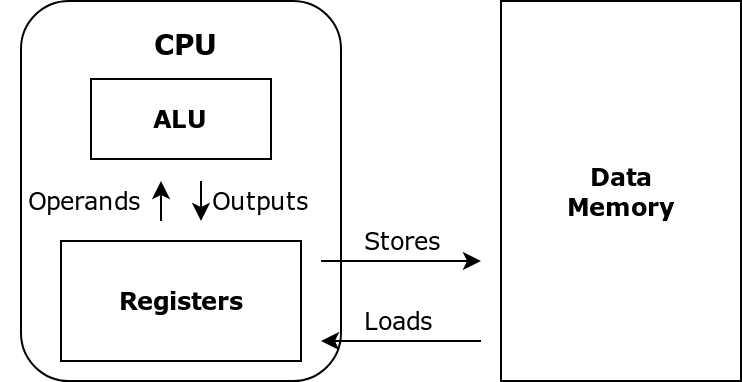
\includegraphics[width=.7\linewidth]{images/simple-stateful-cpu.png}
\caption{Simplified/minimalist diagram of a computer system with registers and data memory.}
\end{figure}

A basic memory heirarchy can be implemented by restricting the ALU's operands to be obtained only from registers, while also restricting loads and stores to data memory to only be accessible through registers.  In our experiments, we implement this model with the small caveat that linear memory addressing is implmented by using the ALU's output as the address at which loads and stores from and to data memory are done.



%%%%%% DESIGN APPROACH %%%%%%
\newpage
\section{Design Approach}
\subsection{Register File Design}
To address the problem of supplying mutable registers to the digital system, a $4 \times 9$ array of machine words is encapsulated within a Veriolog module.  This implements the CPU's register file, supplying a total 4 registers, each capable of persistently storing a 9 bit word\footnote{Note that we take a 9-bit integer to be a machine word here, but the ALU itself operates on 8-bit words.  The 9th bit in the exists to support storing the special ALU flags \texttt{ovf} and \texttt{take\_branch}, without loss of information.}.  In Verilog, the array of words is not exposed directly.  The registers may either be written to one-at-a-time or read from two-at-a-time, but not both simultaneously.  This protection mechanism prevents simultaneous reads and writes from the same address and avoids deadlock.  

The registers are read from by setting the \texttt{RegWrite} input bit low and then supplying the desired addresses (an index $i \in [0, 4)$) to the \texttt{ReadAddr1} and \texttt{ReadAddr2} inputs.  The respective outputs of the register file then expose the contents at the requested addresses.  Note that in our first experiment, the corresponding outputs, \texttt{ReadData1} and \texttt{ReadData2}, are only usasble as ALU operands, and each must be enabled as an input by setting \texttt{AluSrc1} and \texttt{AluSrc2} to $0$.  This must be done because each of the ALU inputs is guarded by a multiplexer: the first multiplexer feeds the value $8'b0$ when it is in the high state, while the other multiplexer feeds an immediate operand from the \texttt{Instr\_i} input when it is in the high state.  In our second experiment, \texttt{ReadData2} does double duty as the value that is written to data memory when a store operation occurs. 

The registers may be written written to by setting the \texttt{RegWrite} input bit high and supplying the desired write address to the \texttt{WriteAddr} input.  The value that is supplied to the \texttt{WriteData} input will then be written to the selected register.

\subsection{Data Memory Design}


%%%%%% RESULTS AND ANALYSIS %%%%%%
\newpage
\section{Results and Analysis}

\subsection{Design Simulation}

\subsubsection{Testbench Simulation for the Register File}
\begin{figure}[h]
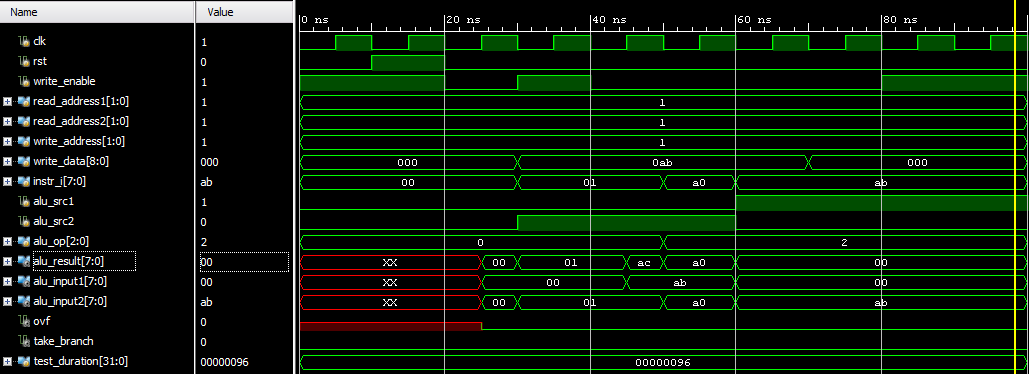
\includegraphics[width=\linewidth]{images/lab4-results-1.png}
\caption{Simulation of the testbench for the register file implementation.}
\end{figure}


\subsection{Hardware Testing}

\FloatBarrier
\subsubsection{Hardware Test Results for the Register File}
\begin{figure}[h]
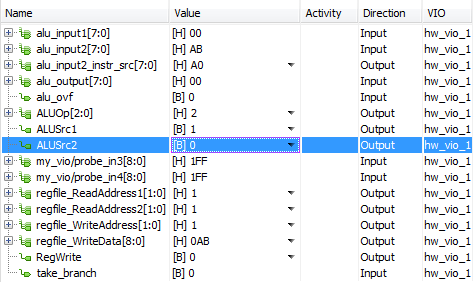
\includegraphics[width=\linewidth]{images/lab4-results-2.png}
\caption{Hardware results for the register file implementation.}
\end{figure}

\FloatBarrier
\subsubsection{Hardware Test Results for the Data Memory Simulation}

\begin{figure}[h]
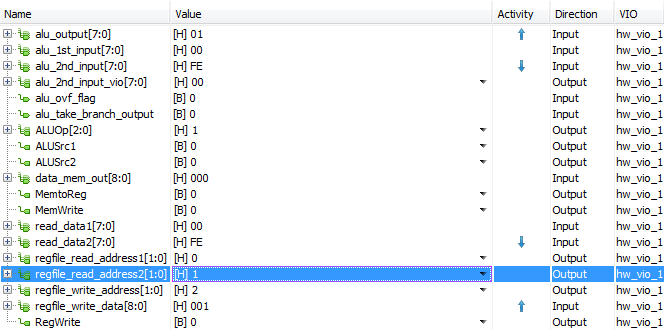
\includegraphics[width=\linewidth]{images/lab5-results-1.png}
\caption{Hardware results for the data memory implementation.  This image shows the desired contents of the first two registers after running the test instruction sequence in the second experiment.}
\end{figure}

\begin{figure}[h]
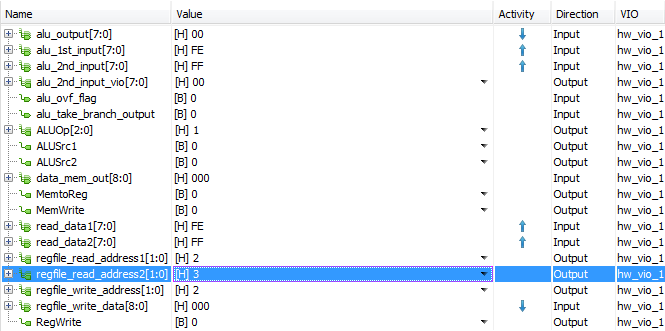
\includegraphics[width=\linewidth]{images/lab5-results-2.png}
\caption{Hardware results for the data memory implementation.  This image shows the desired contents of the last two registers after running the test instruction sequence in the second experiment.}
\end{figure}



%%%%%% CONCLUSIONS %%%%%%

\FloatBarrier\newpage
\section{Conclusions}



%%%%%% APPENDICES %%%%%%
\newpage
\appendix
% explicit 'Appendix' in title before appendix sections
\appendixpage
% explicit 'Appendix' in table of contents
\addappheadtotoc 

\section{\texttt{reg\_file.v}} \label{reg_file_module}
\FloatBarrier
\begin{figure}[h]
	\lstinputlisting[style=verilog-style]{verilog/reg_file.v}
	\caption{\texttt{reg\_file.v} - 4$\times$9 register file implementation in verilog.}
\end{figure}
\FloatBarrier

\section{\texttt{eightbit\_alu.v}} \label{eightbit_alu}
\FloatBarrier
\begin{figure}[h]
	\lstinputlisting[style=verilog-style]{verilog/eightbit_alu.v}
	\caption{\texttt{eightbit\_alu.v} - 8-bit ALU in implementation in verilog.}
\end{figure}
\FloatBarrier


\end{document}
